\documentclass[12pt,pdf]{beamer}
\usepackage[utf8]{inputenc}
\usepackage[russian]{babel}
\usepackage{pscyr}

\usepackage{hedmaths}
\usepackage[quantum]{hedphysics}

\usepackage{graphicx}
\graphicspath{{images//}}

\setbeamertemplate{caption}[numbered]
\usetheme[minimal, numbers, nonav, nologo]{Statmod}
\setbeamerfont{footline}{series=\tiny\bfseries}

\usepackage{tikz}
\renewcommand{\~}[1]{\widetilde{#1}}

\begin{document}
  \begin{frame}
    \begin{center}
    \vspace{3.0cm}
    \normalsize
    \textbf{Квантовая информатика.} \\
    \vspace{1.5cm}
    \raggedleft\small\textbf{Выполнил:}\\Чечеткин~И.~А.\\САПР-1.1п\\
    \vspace{1.8cm}
    \vspace{\fill}
    \centering Волгоград \the\year
    \end{center}
  \end{frame}

  \begin{frame}
    Оглавление:
    \tableofcontents
  \end{frame}

  \section{Введение}
  \begin{frame}
    \frametitle{Введение}
    \begin{figure}
      \center
      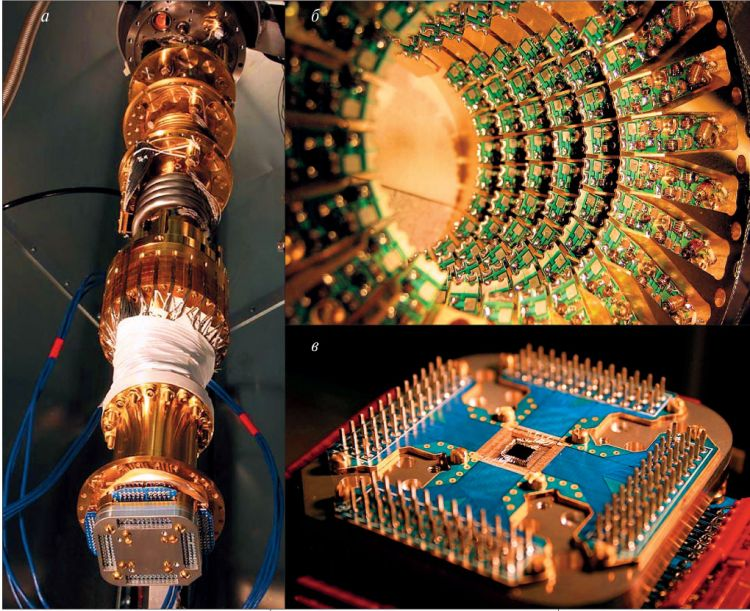
\includegraphics[height=10em]{picture} \hfill
      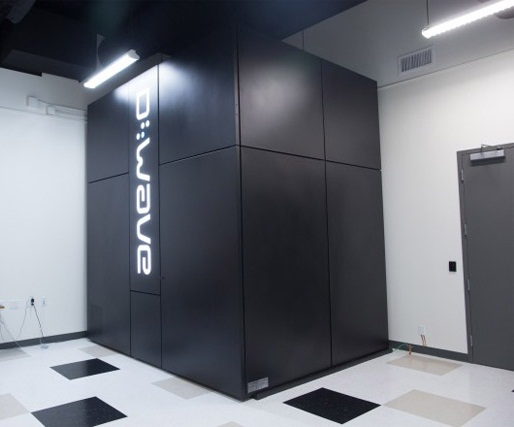
\includegraphics[height=10em]{d-wave}
    \end{figure}
  \end{frame}

  \section{Кубиты}
  \begin{frame}
    \frametitle{Квантовые биты}
    \begin{figure}[h!]
      \center
      \begin{minipage}{.65\textwidth}
        Состояние кубита в общем виде задается волновой функцией вида:
        \[
          \ket\psi = \alpha\ket{0} + \beta\ket{1},
        \]
        где \( \abs{\alpha}^2 + \abs{\beta}^2 = 1 \).
      \end{minipage}
      \begin{minipage}{.3\textwidth}
        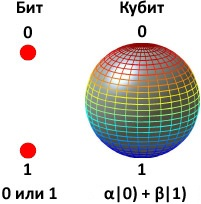
\includegraphics[width=\textwidth]{qubit}
      \end{minipage}
    \end{figure}
    \vspace{.5ex}
    Расписав комплексные коэффициенты \( \alpha \) и \( \beta \), получаем
    представление кубита на сфере Блоха:
    \[
      \ket\psi = \cos\frac{\theta}{2}\ket{0} +
        e^{i\phi}\sin\frac{\theta}{2}\ket{1}.
    \]
    При измерении кубит переходит в одно из состояний \ket{0} или \ket{1}.
  \end{frame}

  \section{Квантовые вентили}
  \begin{frame}
    \frametitle{Квантовые логические элементы}
    \framesubtitle{Однокубитовые вентили}
    \small
    \begin{figure}[h!]
      \center
      \begin{tikzpicture}[scale=.3]
        \draw (0, 2) -- (5, 2);
        \draw (5, 0) rectangle (8, 4);
        \draw (8, 2) -- (13, 2);
        \node at (6.5, 2){\( \hat{U} \)};
        \node [above] at (2.5, 2){\ket{\vphantom{\~\psi}\psi}};
        \node [above] at (10.5, 2){\ket{\~\psi}};
      \end{tikzpicture} \\
      Квантовый процесс вычисления
    \end{figure}
    \vspace{1.5ex}
    \begin{minipage}{.49\textwidth}
      Элементы на матрицах Паули:
      \vspace{-1.5ex}
      \begin{itemize}
        \item элемент X = 
        \( \ds
          \begin{pmatrix}
            0 & 1 \\ 1 & 0
          \end{pmatrix}
        \);
        \item элемент Y = 
        \( \ds
          \begin{pmatrix}
            0 & -i \\ i & 0
          \end{pmatrix}
        \);
        \item элемент Z = 
        \( \ds
          \begin{pmatrix}
            1 & 0 \\ 0 & -1
          \end{pmatrix}
        \).
      \end{itemize}
    \end{minipage}
    \hfill
    \begin{minipage}{.49\textwidth}
      Остальные элементы:
      \vspace{1ex}
      \begin{itemize}
        \item элемент Адамара\\ H = 
        \( \ds
          \frac{1}{\sqrt{2}}
          \begin{pmatrix}
            1 & 1 \\ 1 & -1
          \end{pmatrix}
        \);
        \item элемент сдвига фазы\\ P = 
        \( \ds
          \begin{pmatrix}
            1 & 0 \\ 0 & \exp(i\phi)
          \end{pmatrix}
        \).
      \end{itemize}    
    \end{minipage}  
  \end{frame}
  
  \begin{frame}
    \frametitle{Квантовые логические элементы}
    \framesubtitle{Однокубитовые вентили}
    \footnotesize
    \vspace{-1em}
    \begin{figure}[h!]
      \begin{minipage}{.47\textwidth}
        \center
        \begin{tikzpicture}[scale=.4]
          \draw [->] (4, 0) -- (4, 8) node [left] {\( \beta \)};
          \draw [->] (0, 4) -- (8, 4) node [below] {\( \alpha \)};
          \draw (4, 4) circle [radius=3];
          \draw [->] (4, 4) -- (5, 6.84) node [above] {\ket\psi};
          \draw [very thick] (.5, .5) -- (7.5, 7.5);
          \draw [->] (4, 4) -- (6.84, 5) node [right] {\ket{\~\psi}};
        \end{tikzpicture}\\
        Действие элемента X
      \end{minipage} \hfill
      \begin{minipage}{.47\textwidth}
        \begin{tikzpicture}[scale=.4]
          \draw [->] (4, 0) -- (4, 8) node [left] {\( \beta \)};
          \draw [->] (0, 4) -- (8, 4) node [below] {\( \alpha \)};
          \draw (4, 4) circle [radius=3];
          \draw [->] (4, 4) -- (5, 6.84) node [above] {\ket\psi};
          \draw [very thick] (.5, 4) -- (7.5, 4);
          \draw [->] (4, 4) -- (5, 1.16);
          \node [below right] at (4.4, 3.8) {\ket{\~\psi}};
        \end{tikzpicture}\\
        Действие элемента Z
      \end{minipage} \\
      \begin{minipage}{.47\textwidth}
        \center
        \begin{tikzpicture}[scale=.4]
          \draw [->] (4, 0) -- (4, 8) node [left] {\( \beta \)};
          \draw [->] (0, 4) -- (8, 4) node [below] {\( \alpha \)};
          \draw (4, 4) circle [radius=3];
          \draw [->] (4, 4) -- (5, 6.84) node [above] {\ket\psi};
          \draw [very thick] (1, 2.5) -- (7, 5.5);
          \draw [->] (4, 4) -- (6.84, 3) node [below right] {\ket{\~\psi}};
        \end{tikzpicture}\\
        Действие элемента H
      \end{minipage} \hfill
      \begin{minipage}{.47\textwidth}
        \begin{tikzpicture}[scale=.4]
          \draw [->] (4, 0) -- (4, 8) node [left] {\( Z \)};
          \draw [->] (0, 4) -- (8, 4) node [below] {\( Y \)};
          \draw [->] (6, 6) -- (1, 1) node [below] {\( X \)};
          \draw (4, 4) circle [radius=3];
          \draw (1, 4) to [out=-90, in=-90] (7, 4);
          \draw [dashed] (1, 4) to [out=90, in=90] (7, 4);
          \draw [very thick, ->] (4, 4) -- (4.5, 6);
          \node at (4.5, 6.4) {\ket\psi};
          \draw (4.5, 6) -- (4.5, 2.31) -- (4, 4);
          \draw [very thick, ->] (4, 4) -- (5.75, 6.24);
          \node at (6.5, 7) {\ket{\~\psi}};
          \draw (5.75, 6.24) -- (5.75, 2.55) -- (4, 4);
          \draw [->] (4.27, 3.1) to [out=-20, in=220] (4.97, 3.2);
          \node at (4.9, 2.7) {\( \phi \)};
        \end{tikzpicture}\\
        Действие элемента P
      \end{minipage}
    \end{figure}
  \end{frame}
  
  \begin{frame}
    \frametitle{Квантовые логические элементы}
    \framesubtitle{Двукубитовые вентили}
    \vspace{-1ex}
    \begin{figure}[h!]
      \center
      \begin{tikzpicture}[scale=.3]
        \draw (0, 4) -- (8, 4);
        \draw (0, 0) -- (3, 0);
        \draw (3, -1) rectangle (5, 1);
        \draw (5, 0) -- (8, 0);
        \node at (4, 0){\( U \)};
        \draw (4, 1) -- (4, 4);
        \draw [fill] (4, 4) circle [radius=.15];
      \end{tikzpicture}\\
      \footnotesize Управляемое преобразование
    \end{figure}
    
    \vspace{1ex}
    \begin{minipage}{.4\textwidth}
      \center
      \begin{tikzpicture}[scale=.4]
        \draw (0, 4) -- (8, 4);
        \draw (0, 0) -- (8, 0);
        \draw (4, 0) circle [radius=.5];
        \draw (4, -.5) -- (4, 4);
        \draw [fill] (4, 4) circle [radius=.15];
      \end{tikzpicture}
    \end{minipage}
    \begin{minipage}{.42\textwidth}
      \[
        CNOT =
        \begin{pmatrix}
          1 & 0 & 0 & 0 \\[-.7ex]
          0 & 1 & 0 & 0 \\[-.7ex]
          0 & 0 & 0 & 1 \\[-.7ex]
          0 & 0 & 1 & 0
        \end{pmatrix},
      \]
    \end{minipage}
    
    \begin{minipage}{.4\textwidth}
      \center
      \begin{tikzpicture}[scale=.4]
        \draw (0, 4) -- (8, 4);
        \draw (0, 0) -- (3, 0);
        \draw (3, -1) rectangle (5, 1);
        \draw (5, 0) -- (8, 0);
        \node at (4, 0){\( P \)};
        \draw (4, 1) -- (4, 4);
        \draw [fill] (4, 4) circle [radius=.15];
      \end{tikzpicture}
    \end{minipage}
    \begin{minipage}{.4\textwidth}
      \[
        CP =
        \begin{pmatrix}
          1 & 0 & 0 & 0         \\[-.7ex]
          0 & 1 & 0 & 0         \\[-.7ex]
          0 & 0 & 1 & 0         \\[-.7ex]
          0 & 0 & 0 & e^{i\phi}
        \end{pmatrix}.
      \]
    \end{minipage}
  \end{frame}

  \section{Квантовые вычисления}
  \begin{frame}
    \frametitle{Квантовые вычисления}
    \framesubtitle{В двух словах}
    Квантовый компьютер состоит из квантовых регистров. Вектор вычислительного
    базиса регистра:
    \[
      \ket{x} = \ket{x_{n-1}, x_{n-2}, \ldots, x_1, x_0},
        \text{ где } x_i = \left\{0, 1\right\}.
    \]
    Каждому вектору можно сопоставить двоичное число:
    \[
      x = x_{n-1} 2^{n-1} + x_{n-2} 2^{n-2} + \ldots + x_1 2 + x_0.
    \]
    
    Произвольное состояние квантового регистра:
    \vspace{-1ex}
    \[
      \ket\psi = \sum_{x=0}^{n-1} a_x\ket{x},
        \text{ где } \sum_x \abs{a_x}^2 = 1.
    \]
    
    \vspace{-1ex}
    Таким образом, квантовый регистр может находиться в суперпозиционном
    состоянии: регистр из \( n \) кубитов может содержать \( 2^n \)
    чисел одновременно. Это позволяет выполнить вычисление сразу для всех
    чисел, записанных в регистр, за один прогон.
  \end{frame}

  \begin{frame}
    \frametitle{Квантовые алгоритмы}
    \framesubtitle{Алгоритм Гровера}
    
    Алгоритм Гровера решает задачу перебора, то есть решения уравнения
    \( f(x) = 1 \), где \( f \)~-- логическая функция от \( n \) переменных.
    Классически данная задача требует прямого перебора всех \( N = 2^n \)
    переменных, данный алгоритм находит корень уравнения за \( \pi\sqrt{N}/4 \)
    обращений к функции \( f \) с использованием \( O(n) \) кубитов.
    \begin{figure}[h!]
      \center
      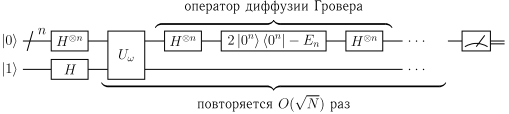
\includegraphics[width=\textwidth]{grover}
    \end{figure}
  \end{frame}
  
  \begin{frame}
    \frametitle{Квантовые алгоритмы}
    \framesubtitle{Алгоритм Шора}
    Алгоритм Шора~-- квантовый алгоритм разложения числа на простые множители,
    позволяющий разложить число \( M \) за время \( O(\lg^3M) \) с
    использованием \( O(\lg M) \) кубитов.
    
    Значимость алгоритма заключается в том, что с его помощью становится
    возможным взлом криптографических систем с открытым ключом.
    \begin{figure}[h!]
      \center
      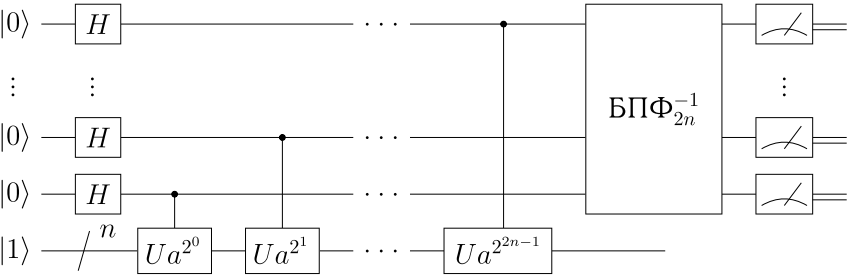
\includegraphics[width=\textwidth]{shor}
    \end{figure}
  \end{frame}
  
  \begin{frame}
    \frametitle{Квантовые алгоритмы}
    \framesubtitle{Алгоритм Дойча--Йожи}
    Задача Дойча--Йожи заключается в определении является ли функция двоичной
    переменной \( f(n) \) постоянной (принимает либо значение 0, либо 1 при
    любых аргументах) или сбалансированной (для половины области определения
    принимает значение 0, для другой половины 1). При этом заранее считается
    известным, что функция либо является константой, либо сбалансирована.
    \begin{figure}[h!]
      \center
      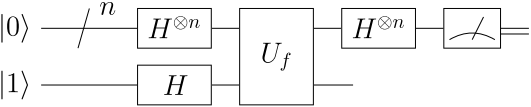
\includegraphics[width=.75\textwidth]{deutch}
    \end{figure}
  \end{frame}
  
  \section{Компьютер D-Wave}
  \begin{frame}
    \frametitle{Компьютер D-Wave}
    \begin{figure}
      \begin{minipage}{.6\textwidth}
        На сегодняшний день существуют ограниченные квантовые компьютеры.
      
        Больших успехов добилась компания D-Wave, создавшая в 2012 образец
        квантового компьютера на основе процессора из 512 кубит~-- D-Wave One.
      \end{minipage}
      \hfill
      \begin{minipage}{.35\textwidth}
        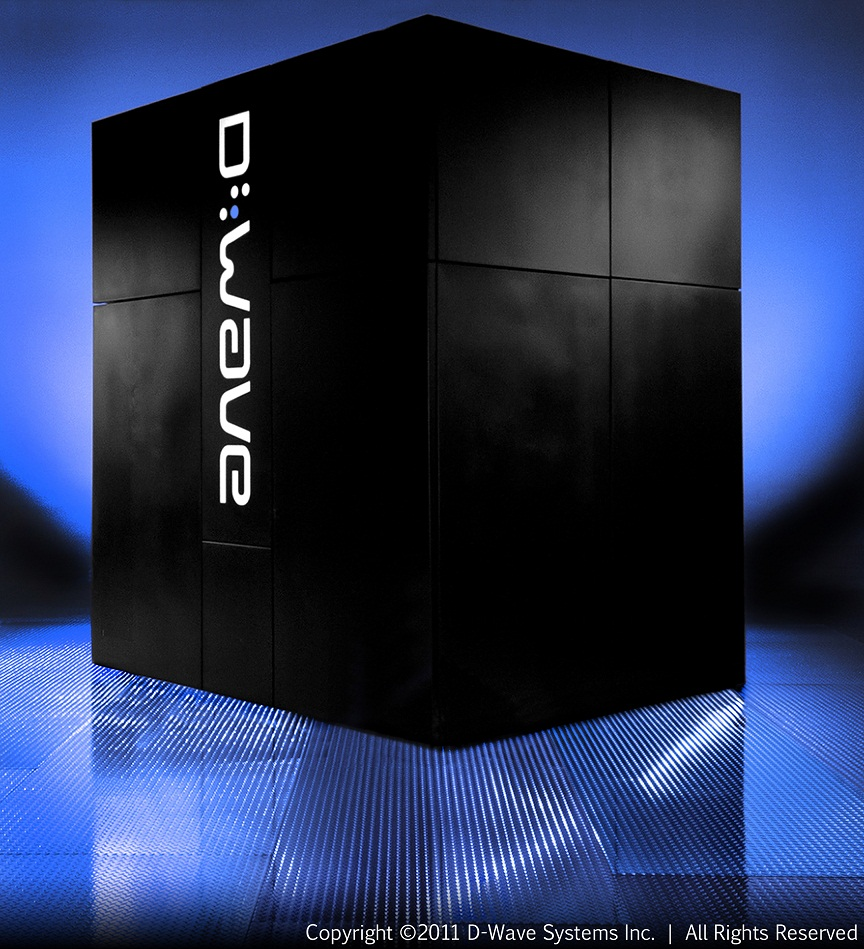
\includegraphics[width=\textwidth]{d-wave_blue}
      \end{minipage}
    \end{figure}
    
    D-Wave One решает задачи методом квантового отжига, поэтому прирост
    скорости решения наблюдается для некоторых специфичных задач:
    задач моделирования динамики сложных систем и задач перебора.
  \end{frame}

  \begin{frame}
    \Huge\centering Спасибо за внимание!
  \end{frame}
\end{document}
